\documentclass[preprint,12pt]{elsarticle}

\usepackage[T1]{fontenc}
\usepackage{lineno}
\usepackage{graphicx}
\usepackage{booktabs}
\usepackage{amsmath}
\usepackage{array}
\usepackage[table]{xcolor}
\usepackage{url}
\usepackage[hidelinks]{hyperref}
\usepackage{caption}
\captionsetup{font=small,labelfont=bf}
\usepackage{ragged2e}
\newcolumntype{L}[1]{>{\RaggedRight\arraybackslash}p{#1}}
\journal{Journal of Biomedical Informatics}

\begin{document}

\begin{frontmatter}

\title{Same ceiling, different machinery: mechanistic interpretability of a text
language model trained to read cells as sentences}

\author[tue]{Ihor Kendiukhov}
\ead{ihor.kendiukhov@student.uni-tuebingen.de}
\affiliation[tue]{organization={Institute of Medical Genetics and Applied Genomics,
                  University of Tübingen}, city={Tübingen}, country={Germany}}

\begin{abstract}
\textbf{Objective.} Single-cell foundation models are increasingly proposed for target
prioritisation and perturbation prediction, yet are judged by benchmark scores that cannot
separate genuine biological computation from a re-encoding of the input. A new class represents a
cell as a \emph{sentence} of gene names, trained as a general-purpose language model. We asked what
such a model internally computes, and sought a reusable protocol for any biomedical foundation
model.

\textbf{Methods.} We applied a four-stage protocol to C2S-Scale, a Cell2Sentence family built on
Gemma-2 (2B and 27B). We trained per-layer TopK sparse autoencoders on gene-token activations,
annotated features against Gene Ontology, KEGG, Reactome, STRING and TRRUST, traced causal circuits
by feature ablation, and tested whether the geometry exceeds co-expression and is causally used,
via permutation nulls and activation steering. Three controls applied throughout: baselines encoded
with the model's own input information, nulls matched on co-expression, and capacity-matched
comparison across sizes.

\textbf{Results.} The models carry extensive biologically organised structure: 68\% of features
received a significant ontology annotation; half of the layer-0 features remained recoverable at
layer 25, versus 2--3\% for an encoder-style model under the same pipeline; 27,633 causal
cross-layer edges were recovered, 85.2\% joining features sharing an ontology term; and functional
relatedness exceeded a co-expression-matched null ($z = 3.9$--$6.6$). Steering internal directions
moved the model's own predictions; random directions did not. Two negatives were equally robust:
gene knockdowns were detected for 96.7\% of targets but only 2.1\% produced a
transcription-factor-target-specific response, and at matched capacity the 27B model had 31 times
more dead features and 19 points lower annotation than the 2B.

\textbf{Conclusion.} Cell-sentence language models build rich, causally used, largely interpretable
structure, but it encodes co-expression rather than regulatory direction, and scale does not
improve it. The protocol and a public feature atlas are released for assessing other biomedical
foundation models.
\end{abstract}

\begin{keyword}
foundation models \sep interpretability \sep sparse autoencoders \sep single-cell transcriptomics
\sep model evaluation \sep causal analysis
\end{keyword}

\end{frontmatter}

\section{Introduction}

Foundation models trained on large single-cell transcriptomic corpora are now being proposed for
tasks with direct translational consequence: prioritising drug targets, predicting the effect of a
genetic perturbation, and annotating cells in diseased human tissue \cite{ref3,ref4}. Decisions
taken on the strength of such predictions are only as trustworthy as our understanding of what the
model has actually learned. That understanding is currently thin. Most evaluations report a
downstream accuracy, and accuracy alone cannot separate a model that has internalised gene
regulation from one that has efficiently re-described the correlations already present in its
input.

This gap matters because the dominant statistical structure in transcriptomic data --- genes that
are expressed together --- can imitate almost any biological signal one might wish to claim. A model
that reproduces co-expression will appear to ``know'' pathways, cell types and cell states, because
those categories are themselves largely defined by co-expression. Prior work across several
architectures has repeatedly found that apparent regulatory knowledge in these models collapses
once co-expression is properly controlled \cite{ref8,ref9}. Evaluation therefore needs to be
supplemented by interpretability: methods that open the model and ask which internal quantities
exist, how they are connected, whether they are used, and whether any of it exceeds the information
already handed to the model at its input.

A recent and distinctive class of single-cell models makes this question sharper. Cell2Sentence
\cite{ref1} represents a cell as a \emph{sentence}: the genes are sorted by expression and written
out as a plain list of gene symbols, so that a general-purpose language model can be trained on
cells exactly as it would be trained on text. C2S-Scale \cite{ref2} scales this idea to billions of
parameters on the Gemma-2 architecture. Such a model is architecturally a text transformer, has no
learned gene-embedding table of the kind found in encoder-style single-cell models, and ---
importantly --- discards expression magnitudes, retaining only which genes are present and in what
order. It is therefore an unusually clean testbed: whatever the model contributes must be visible as
a difference between the model and its own input encoding.

We report a mechanistic-interpretability study of this model class, and, as the methodological
contribution, the protocol used to obtain it. The protocol has four stages (Fig.~\ref{fig:design})
--- a sparse-autoencoder feature atlas, causal circuit tracing, geometry and steering tests, and
public deployment of the resulting atlas --- and is bound together by three controls that we argue
should be standard: (i) \textbf{information-matched baselines}, in which the comparison baseline is
encoded with exactly the information the model receives; (ii) \textbf{co-expression-matched nulls},
in which the null distribution preserves the co-expression structure of the same cells; and (iii)
\textbf{capacity-matched scaling controls}, in which interpretability is compared across model sizes
only after equalising the number of features per unit of training data. Each of these controls
changed a conclusion in this study, in one case reversing it.

We apply the protocol to C2S-Scale at 2B and 27B parameters, using human chronic myeloid leukaemia
cells (K562) with genome-scale CRISPR interference \cite{ref24} and human bone-marrow CD34+
haematopoietic progenitors \cite{ref25}. We report both positive and negative findings, and we
release the feature atlas as a public, browsable resource.

\begin{table}[htbp]
\centering
\caption{Statement of Significance.}
\label{tab:sos}
\small
\begin{tabular}{@{}L{0.24\linewidth}L{0.70\linewidth}@{}}
\toprule
\textbf{Problem or Issue} & Single-cell foundation models are being adopted for translational tasks, but are evaluated by benchmark accuracy, which cannot distinguish learned biology from a re-encoding of the model's own input. \\
\midrule
\textbf{What is Already Known} & Sparse autoencoders extract interpretable features from encoder-style single-cell models, whose attention largely reflects co-expression rather than regulation. Nothing is known about the internals of models that read a cell as a sentence of gene names. \\
\midrule
\textbf{What this Paper Adds} & A four-stage interpretability protocol with three transferable controls (information-matched baselines, co-expression-matched nulls, capacity-matched scaling), applied to a cell-sentence language model at two scales. It finds extensive, causally used interpretable structure, no transcription-factor-to-target regulatory logic, and that scaling to 27B parameters reduces interpretability. A public feature atlas is released. \\
\midrule
\textbf{Who would benefit} & Developers and evaluators of biomedical foundation models; computational biologists judging whether such models can be trusted for target or perturbation reasoning; interpretability researchers. \\
\bottomrule
\end{tabular}
\end{table}

\section{Related Work}

\textbf{Sparse autoencoders for language models.} Sparse dictionary learning on transformer
activations recovers directions that are more interpretable than individual neurons, addressing
superposition, in which a network represents more concepts than it has dimensions \cite{ref21}. This
line of work established that features found this way are monosemantic and manipulable
\cite{ref17,ref18,ref19}, and that a TopK constraint gives a clean sparsity--fidelity trade-off with
a single interpretable hyperparameter \cite{ref20}. We adopt the TopK formulation.

\textbf{Interpretability of single-cell foundation models.} Sparse autoencoders have been applied to
encoder-style single-cell models, recovering cell-type and pathway programmes \cite{ref6} and, in a
comparative atlas of Geneformer and scGPT, organised biological knowledge together with a
conspicuous absence of regulatory logic \cite{ref7}. Causal circuit tracing has been used to compare
computational architectures across such models \cite{ref10}, and extended to exhaustive mapping
\cite{ref11}. Complementary studies show that attention-derived scores mainly re-encode
co-expression and add little over simple gene-level features for perturbation-target prediction
\cite{ref8,ref9}, and that geometric and topological structure in these models is extensive but
frequently explicable by data structure \cite{ref12,ref13,ref37}. Intervention-based validation of
putative regulatory signal has been formalised separately \cite{ref14}. The present work carries
this programme to a model class it has not previously reached, and adds the capacity-matched scaling
control.

\textbf{Cell-sentence models.} Cell2Sentence \cite{ref1} introduced the rank-ordered gene-name
representation and showed that language models fine-tuned on it can generate and annotate cells;
C2S-Scale \cite{ref2} scaled this to 27B parameters. Independently, zero-shot evaluations have
questioned how much single-cell foundation models add over simple baselines \cite{ref5}, which is
precisely the question our information-matched baselines are designed to answer.

\textbf{Evaluation validity.} Benchmark rankings for these models are unstable under protocol
choices and are bounded by partial-label ceilings \cite{ref39,ref40}. This motivates our emphasis on
controls rather than on leaderboard position.

\section{Methods}

\subsection{Models, data and input construction}
We studied C2S-Scale \cite{ref2} built on Gemma-2 \cite{ref23}: the 2B variant (26 transformer
layers, hidden width 2304) and the 27B variant (46 layers, width 4608). Both use a shared
20,275-token vocabulary and were accessed as HuggingFace \texttt{safetensors} checkpoints so that
hidden states could be captured with standard hooks.

A cell is converted to a sentence by ranking genes by expression and emitting the top 512 gene
symbols in order; expression magnitudes are discarded. Because a gene symbol may span several
sub-word tokens, we mapped tokens back to genes using the tokenizer's character offsets and
mean-pooled the residual stream over the tokens of each gene, yielding one activation vector per
(cell, gene) pair, which we call a \emph{gene-token position}. Scaffold tokens (prompt and
punctuation) were excluded.

Two human datasets were used. For the atlas, circuit tracing and the regulatory-logic test we used
K562 cells from a genome-scale CRISPR-interference Perturb-seq experiment \cite{ref24}; the atlas
used 1,200 unperturbed cells (614,400 gene-token positions per layer) and the regulatory-logic test
used the full essential-gene screen. For the geometry analyses we used CD34+ human bone-marrow
progenitors with diffusion-pseudotime and lineage labels \cite{ref25}.

\subsection{Stage 1 --- sparse-autoencoder feature atlas}
For each layer we trained a TopK sparse autoencoder \cite{ref20} on the gene-token activations:
dictionary size 9,216 ($4\times$ the 2B width), $k = 32$ active features per position, 6 epochs,
with decoder columns constrained to unit norm. Two implementation details proved load-bearing.
First, the unit-norm constraint must be applied along the \emph{feature} axis; normalising the wrong
axis silently killed 34.8\% of features. Second, activations must be stored in 32-bit precision for
the 27B model, whose late-layer activations exceed the range of 16-bit floats and otherwise produce
non-finite values.

Each feature was summarised by its activation frequency, mean activation and the genes that most
strongly drive it. Features were annotated by testing the overlap between a feature's top genes and
Gene Ontology biological processes \cite{ref41,ref42}, KEGG pathways \cite{ref43,ref44}, Reactome
pathways \cite{ref45}, STRING interaction neighbourhoods \cite{ref46} and TRRUST
transcription-factor target sets \cite{ref47}, using Fisher's exact test with Benjamini--Hochberg
control of the false discovery rate \cite{ref34}. Co-activation modules were obtained by Leiden
clustering \cite{ref32} of the feature co-activation graph. To quantify how features change with
depth we matched features between layers by decoder cosine similarity and recorded the fraction of
layer-0 features still recoverable at each later layer.

\subsection{Stage 2 --- causal circuit tracing}
For a chosen source layer we selected the highest-scoring annotated features and, for each, ran a
clean forward pass and an ablated forward pass in which that feature's contribution was removed from
the residual stream, using a forward hook, in the spirit of activation patching in language models
\cite{ref22}. We then measured the change in every downstream layer's feature activations,
accumulating means and variances online. An edge was recorded when the standardised effect was
significant and consistent across cells. Because the full design (200 cells $\times$ 30 features
$\times$ 3 layers, an unbatched pass per pair) required roughly 15--20\,h on the available hardware,
we ran a reduced but complete design: 50 cells and 15 features at source layers 0, 7 and 16.

\subsection{Regulatory-logic test}
We asked whether an internal feature encodes the direction of regulation rather than mere
association. For each of 48 TRRUST transcription factors and 12 non-transcription-factor controls we
compared 25 knockdown cells against 400 non-targeting control cells. A feature was \emph{responding}
if its activation differed between conditions (Mann--Whitney $U$, BH-corrected). A transcription
factor showed \emph{specific} response if the genes driving its responding features overlapped that
factor's known targets more than expected (Fisher's exact test, BH-corrected across factors).

\subsection{Capacity-matched scaling control}
Comparing interpretability across model sizes is confounded: at a fixed expansion factor the wider
model receives a proportionally larger dictionary trained on the same number of positions, so its
features are systematically under-trained. We therefore retrained the 27B autoencoders at an
expansion factor of 2, giving 9,216 features --- the same absolute dictionary as the 2B model and
hence the same ${\sim}67$ positions per feature --- and repeated the catalogue and annotation steps.

\subsection{Stage 3 --- geometry, nulls and steering}
To ask whether the model's gene geometry encodes function beyond co-expression, we binned gene pairs
jointly on co-expression and mean expression and measured, within bins, how much more
cosine-similar same-function pairs are than different-function pairs. Because the binning already
matches co-expression, the appropriate null permutes the assignment of functional labels to genes;
we drew 200 such permutations and report a $z$-score against them. Intrinsic dimensionality was
estimated by participation ratio and by the TwoNN estimator.

For cell-state geometry we compared the model's representation with a principal-component embedding
of the raw counts of the \emph{same} cells, matched on dimensionality, scoring pseudotime recovery,
curvature (the gain of a nearest-neighbour regressor over a linear one) and lineage recovery.

Causal use was tested by activation steering \cite{ref48,ref49}: internal states were displaced
along a target direction and the model's own next-gene predictions were read out, against a
norm-matched random direction as control.

\subsection{Information-matched baselines}
Every model-versus-data comparison used a baseline given exactly the information the model receives.
Because a cell sentence is the top-512 genes in rank order without magnitudes, the correct baseline
is not the full expression vector but the same truncated, rank-only encoding. We report the full
ladder (full expression, top-512 with magnitudes, top-512 as a binary set, top-512 set plus rank) so
that the cost of tokenisation is separated from the contribution of the model.

\subsection{Implementation}
Experiments ran on rented NVIDIA A40, A5000, RTX 4090 and A100/H100 GPUs. Code, trained
autoencoders and result artefacts are available as described in Data Availability.

\section{Results}

\subsection{The model carries a large, biologically annotated feature dictionary}
Sparse autoencoders trained on all 26 layers of the 2B model reconstructed the residual stream well,
explaining 87--99\% of activation variance (mean 0.93), with few dead features (mean 1.2\%) and
near-orthogonal decoder directions (mean absolute cosine 0.02) (Fig.~\ref{fig:atlas}a). On average
68\% of features per layer received at least one significant ontology annotation, ranging from 80\%
in early layers to about 50\% late (Fig.~\ref{fig:atlas}b), and 16--26 co-activation modules were
recovered per layer. Feature contents were recognisable cell-biological programmes --- ribosomal
subunits (with the large and small subunits separated), proteasome, spliceosome, chaperonin,
translation initiation, mitosis and glycolysis --- consistent with a proliferating leukaemia line.

Almost no feature aligned with a top-50 singular direction of the same activations (0--1 per layer;
99.99\% of features novel), reproducing in a cell-sentence model the observation that sparse
features are not visible to linear decomposition \cite{ref7,ref21}.

\subsection{Features persist across the entire depth}
Tracking features by decoder similarity, 63\% of layer-0 features were still recoverable more than
ten layers later, and 50.4\% remained at layer 25 with mean cosine 0.88
(Fig.~\ref{fig:atlas}c). Under the identical pipeline, an encoder-style single-cell model retains
2--3\% and nothing beyond layer 11 \cite{ref7}. A decoder-only residual stream therefore preserves
gene-level feature directions written early, whereas encoder-style single-cell models rebuild their
features layer by layer. This is an architecture-level contrast with a practical consequence: in
this model class, a feature discovered at one depth can be expected to remain addressable at others.

\subsection{Causal circuits propagate biological function}
Ablating individual features and measuring downstream consequences yielded 27,633 significant
cross-layer edges from 45 source features to 7,959 distinct downstream features. Influence
attenuated smoothly with distance, from 746 edges into the adjacent layer to 196 into the last
(Fig.~\ref{fig:circuits}a), with no long-range anomalies. Of the 12,816 edges for which both
endpoints were annotated, 10,919 (85.2\%) connected features sharing at least one ontology term
(Fig.~\ref{fig:circuits}b). Typical circuits propagate a single function across depth: a
DNA-damage-response feature at layer 7 drives DNA-damage-response features at layers 8, 12, 14 and
22.

This is coherent, interpretable computation. It is not, by itself, evidence of regulatory logic:
features sharing an ontology term are annotated from overlapping and largely co-expressed gene sets,
so functional propagation is what co-expression alone predicts.

\subsection{The model detects perturbations but does not encode regulatory direction}
The regulatory-logic test separates these possibilities. The model registered the knockdown for
96.7\% of targets (58/60): individual transcription factors shifted hundreds of features. Yet only
2.1\% of transcription factors (1 of 48, BH $q < 0.05$) produced a response whose driving genes were
enriched for that factor's known targets (Fig.~\ref{fig:circuits}c) --- at the false-discovery
floor, and statistically indistinguishable from zero. An encoder-style reference model under the
same test reaches 6.2\% \cite{ref7}.

Near-perfect detection with null specificity is the signature of a model that has learned which
genes move together, not which gene controls which. Scaling from encoder-style single-cell models to
a 2B-parameter generative language model trained on tens of millions of cells did not purchase
regulatory logic.

\subsection{Scale reduces interpretability, and the confound is only partly responsible}
At its native $4\times$ expansion the 27B model looked markedly less interpretable than the 2B:
47.5\% dead features against 1.2\%, and 44.9\% of live features annotated against 73.4\%. This
comparison is confounded, because the wider model's dictionary is twice as large on the same data.
Retraining the 27B autoencoders at matched dictionary size recovered roughly ten points on each
measure (dead 47.5\% $\rightarrow$ 37.7\%; annotation 44.9\% $\rightarrow$ 54.5\%), confirming that
under-training was a real effect worth controlling.

It did not explain the gap. At matched capacity and matched positions per feature, the 27B model
still had 37.7\% dead features against the 2B model's 1.2\% --- a factor of 31 --- and 19 percentage
points lower annotation among live features (Fig.~\ref{fig:scaling}). The 27B model simultaneously
achieved \emph{higher} reconstruction fidelity (0.977 against 0.933) using far fewer live features,
indicating a more anisotropic residual stream in which computation concentrates in fewer, denser and
less ontology-aligned directions. In this model family, thirteen times the parameters made the
internals harder to read, not easier.

\subsection{Gene geometry exceeds co-expression; cell-state geometry does not}
Gene representations were high-dimensional (participation ratio 94--132; TwoNN estimate 5.0--6.2).
Within bins matched on co-expression and mean expression, functionally related gene pairs were more
aligned than unrelated pairs by $\Delta\cos = 0.062$, 0.044 and 0.055 at layers 9, 13 and 17.
Against 200 label permutations the null sat at approximately zero, and the observed values cleared
it at $z = 6.57$, 3.86 and 4.52 ($p \le 0.01$) (Fig.~\ref{fig:beyond}a). This is a genuine, if
modest, signal beyond co-expression, strongest in mid-network layers.

The cell-level result went the other way. The model does embed the haematopoietic trajectory as a
curved manifold, recovering pseudotime ($R^2 = 0.70$) and lineage (balanced accuracy 0.605 against a
0.107 chance level), and its curvature exceeds a decodability-matched linear control. But a
principal-component embedding of the raw counts of the same cells did all of it better (pseudotime
$R^2$ 0.86; curvature 0.102 against 0.023; lineage accuracy 0.862). At the level of cell state, the
representation adds no trajectory geometry beyond expression.

\subsection{Internal directions are causally used}
Interpretability claims are strengthened when the identified structure is shown to drive behaviour.
Steering the residual stream along an internal cell-state direction moved the model's own next-gene
predictions by approximately 0.8\,rad toward the target state, while a norm-matched random direction
produced essentially no movement (0.007). Comparing steering rules, displacement along the local
geometry of the representation produced a longer traversal of the model's readout than a fixed
linear direction in three independent runs (1.97/0.93/2.29\,rad against 0.95/0.47/1.32; 75--92\% of
cells; $p$ between $1\times10^{-5}$ and 0.01) (Fig.~\ref{fig:beyond}b). The internal geometry is
therefore not decorative: the model's outputs follow the path along which its states are moved.

\subsection{On cell-level tasks the model does not exceed its own input}
Placing the model and its baselines on one ruler, recovery of a cell-state variable was 0.929 from
full expression with magnitudes, 0.882 from the top-512 genes as a binary set, 0.875 from the model,
and 0.868 from the same set plus rank (Fig.~\ref{fig:beyond}c). Almost the entire loss relative to
full expression ($-0.047$) occurs at tokenisation, when magnitudes are discarded; the model itself
sits within 0.007 of a linear readout of its own input. In a matched benchmark across layers and
embedding dimensionalities, the model did not exceed the expression baseline in any of 36
comparisons.

An important qualification prevents this from being read as ``the model learns nothing''. When the
model is given a gene \emph{name} alone, on a phase-neutral background where no expression
covariance is available, it still sorts genes by the cell-cycle phase they belong to (AUROC 0.989),
whereas an anagram of the same letters performs at chance (0.511); the effect survives residualising
on symbol length, abundance and detection rate (0.908). The mapping from gene name to biological
role is in the weights, even though the cell-level representation is largely a re-encoding of the
input.

\subsection{A public feature atlas}
The final protocol stage deploys the atlas as a browsable resource: 13 layers, 119,808 features,
88,137 with ontology annotations, 188 co-activation modules, with per-feature gene loadings,
enrichments, UMAP layouts \cite{ref50}, cross-layer flow and causal edges, at
\url{https://biodyn-ai.github.io/c2s-atlas/}.

\begin{table}[htbp]
\centering
\caption{The protocol as executed. Positions are gene-token activations; one position is one
(cell, gene) pair.}
\label{tab:grid}
\footnotesize
\begin{tabular}{@{}L{0.17\linewidth}L{0.15\linewidth}L{0.15\linewidth}L{0.22\linewidth}L{0.23\linewidth}@{}}
\toprule
\textbf{Stage} & \textbf{Model} & \textbf{Data} & \textbf{Scale of run} & \textbf{Primary output} \\
\midrule
1. Feature atlas & C2S-2B, all 26 layers & K562, 1,200 cells & 614,400 positions/layer; 9,216
features/layer & 239,616 features; catalogues, annotations, modules \\
1. Feature atlas & C2S-27B, 26 of 46 layers & K562, 1,200 cells & 614,400 positions/layer &
Scaling comparison \\
1b. Capacity-matched control & C2S-27B, 26 layers & K562 & 9,216 features/layer ($2\times$
expansion) & Confound-corrected scaling verdict \\
2. Circuit tracing & C2S-2B, sources L0/L7/L16 & K562, 50 cells & 15 features/source; 800 forward
passes/source & 27,633 causal edges \\
2b. Regulatory-logic test & C2S-2B, L16 & K562 CRISPRi, 60 targets & 25 cells/target vs.\ 400
controls & Detection and specificity rates \\
3. Gene geometry $+$ null & C2S-2B, L9/L13/L17 & CD34+, 4,000 cells & 2.03M positions; 200
permutations & Beyond-co-expression $z$-scores \\
3. Cell-state geometry & C2S-2B, L18 & CD34+, 3,000 cells & Matched 20-D comparison & Model vs.\
expression-PCA verdict \\
3. Steering & C2S-2B & K562 & 3 runs; 12--32 cells/run & Causal-use test \\
4. Deployment & C2S-2B, 13 layers & --- & 119,808 features & Public web atlas \\
\bottomrule
\end{tabular}
\end{table}

\begin{table}[htbp]
\centering
\caption{Summary of findings. Each claim is paired with the control that makes it interpretable.}
\label{tab:findings}
\footnotesize
\begin{tabular}{@{}L{0.27\linewidth}L{0.22\linewidth}L{0.28\linewidth}L{0.16\linewidth}@{}}
\toprule
\textbf{Finding} & \textbf{Statistic} & \textbf{Control applied} & \textbf{Verdict} \\
\midrule
Features are biologically annotated & 68\% of features per layer (mean) & BH-corrected Fisher tests
& Positive \\
Features persist across depth & 50.4\% of L0 features at L25, cosine 0.88 & Same pipeline on an
encoder model (2--3\%) & Positive \\
Circuits propagate function & 85.2\% of annotated edges share a term & Attenuation profile; ontology
annotation & Positive, but co-expression-compatible \\
Gene geometry beyond co-expression & $\Delta\cos$ 0.044--0.062, $z = 3.9$--$6.6$ & 200
co-expression-matched label permutations & Positive \\
Internal directions are causally used & Own-logit shift 0.82\,rad vs.\ 0.007 & Norm-matched random
direction & Positive \\
Regulatory (TF$\rightarrow$target) logic & 2.1\% specific vs.\ 96.7\% detection & BH across factors;
non-TF controls & Negative \\
Scale improves interpretability & 37.7\% vs.\ 1.2\% dead at matched capacity & Capacity-matched
retraining & Negative \\
Cell-state geometry beats expression & Curvature 0.023 vs.\ 0.102 & Matched-dimension expression PCA
& Negative \\
Cell-level task performance beats input & 0.875 vs.\ 0.882 (set) / 0.929 (full) &
Information-matched encoding ladder & Negative \\
\bottomrule
\end{tabular}
\end{table}

\section{Discussion}

Read together, the results describe a model that has learned a great deal about \emph{which genes
belong together} and very little about \emph{which gene controls which}. The evidence for the first
is strong and comes from several independent directions: an extensive dictionary of annotated
features, coherent causal circuits that propagate function across depth, gene geometry that exceeds
a co-expression-matched null, and internal directions whose manipulation changes the model's own
predictions. The evidence for the second is a clean and well-powered negative: near-perfect
detection of gene knockdowns combined with essentially no transcription-factor-target specificity.

This distinction has direct translational consequence. A model of this kind is a reasonable
instrument for describing and organising cell state, and its features are usable as an interpretable
vocabulary for that purpose. It is not a safe basis for claims of the form ``perturbing gene A will
act through target B'', which is precisely the form of claim most attractive in target discovery.
Our results suggest such claims would be supported by co-expression structure rather than by learned
regulation, and would fail in exactly the cases --- novel or non-co-expressed regulatory
relationships --- where a model would be most valuable.

The scaling result deserves separate emphasis because it runs against a common assumption. Larger
models are widely expected to be more capable and, implicitly, more legible. Here the opposite held:
after removing the under-training confound, the 27B model retained 31 times more dead features and
19 points lower annotation than the 2B model, while reconstructing its activations \emph{better}
with fewer live features. The natural reading is increased anisotropy: computation concentrates in
fewer, denser directions that align less well with curated biological categories. For practitioners
this means an interpretability budget is not automatically better spent on the largest available
model, and for the field it means interpretability of biomedical foundation models should be
measured, not assumed to follow capability.

The most transferable part of this work is the control discipline, because each control changed a
conclusion. The information-matched baseline was decisive: an earlier analysis appeared to show the
model sharpening a biological signal roughly three-fold over its own input, but that gap was an
artefact of how we had encoded the baseline; encoding the baseline with exactly the information the
model receives reduced the model's advantage to 0.007. The co-expression-matched null converted an
ungated descriptive observation into a significant finding in one case and dissolved apparent
structure in others. The capacity-matched scaling control recovered ten points of apparent
interpretability that were pure artefact, while leaving a real effect intact. We recommend all three
as routine practice for interpretability claims about biomedical foundation models, and we note that
the same logic --- match the baseline to the model's input, match the null to the data's dominant
correlation structure, match capacity before comparing sizes --- applies equally to models of
clinical text or medical images.

Finally, one asymmetry is worth highlighting because it is easy to miss. Although the model's
\emph{cell-level} representation is close to a re-encoding of its input, the mapping from a gene's
\emph{name} to its biological role is clearly in the weights: given only a gene symbol on a neutral
background, the model sorts genes by cell-cycle phase at AUROC 0.989 while a letter-scrambled
control performs at chance. Language pretraining has left real biological knowledge in the model
that is not present in any single input; the limitation is in what the model does with a cell, not
in what it knows about a gene.

\subsection{Limitations}
The atlas, circuit tracing and regulatory-logic test used one human cell line (K562), so feature
contents are biased toward a proliferative phenotype; the geometry analyses used one progenitor
tissue. Circuit tracing was run at reduced scope (50 cells, 15 features, three source layers)
because the unbatched design is computationally expensive; effect sizes should be read as indicative
and the design does not exhaust the circuit. The 27B atlas covers 26 of 46 layers. Two layers were
excluded from the public atlas because their stored catalogues were corrupted. Ontology annotation
is subject to database circularity; our permutation nulls neutralise this for the comparative claims
but not for absolute annotation rates. Steering was tested on a small number of cells and on a
limited set of internal variables. Finally, all claims concern this model family; the protocol, not
the specific numbers, is what we expect to transfer.

\section{Conclusion}

We have described a four-stage mechanistic-interpretability protocol for biomedical foundation
models and applied it to a language model that reads a cell as a sentence of gene names. The model
builds an extensive, biologically annotated and causally used internal vocabulary whose features,
unusually, persist across its entire depth; its gene geometry encodes functional relatedness beyond
co-expression; and, given only a gene name, it demonstrably knows something about that gene's role.
At the same time it does not represent the direction of gene regulation, it does not exceed a
properly encoded baseline on cell-level tasks, and scaling it thirteen-fold made its internals less
rather than more interpretable.

\textbf{Applicability.} For groups building or selecting single-cell foundation models, the protocol
provides a concrete, reusable procedure --- with three specific controls --- for deciding what a
model can be trusted to do before it informs a biological or clinical decision. For groups using
such models, the immediate practical guidance is to treat their outputs as statements about
co-expression rather than regulation, to prefer smaller models when internal legibility matters, and
to benchmark against baselines encoded with the model's own input. The released feature atlas allows
any of the features reported here to be inspected directly, and the protocol can be applied
unchanged to other model families.

\section*{Declaration of competing interest}
The author declares no competing financial interests or personal relationships that could have
appeared to influence the work reported in this paper.

\section*{Funding}
This research did not receive any specific grant from funding agencies in the public, commercial, or
not-for-profit sectors.

\section*{CRediT authorship contribution statement}
\textbf{Ihor Kendiukhov:} Conceptualization, Methodology, Software, Formal analysis, Investigation,
Data curation, Writing -- original draft, Writing -- review and editing, Visualization, Project
administration.

\section*{Data availability}
The single-cell datasets analysed are publicly available: genome-scale Perturb-seq in K562
\cite{ref24} and CD34+ bone-marrow progenitors \cite{ref25}. Model weights are publicly available
from the model authors \cite{ref2}. Code, trained sparse autoencoders, feature catalogues,
annotations and causal-edge tables generated in this study are accessible through the interactive
atlas at \url{https://biodyn-ai.github.io/c2s-atlas/} and its source repository
\url{https://github.com/Biodyn-AI/c2s-atlas}.

\section*{Declaration of generative AI and AI-assisted technologies in the manuscript preparation
process}
During the preparation of this work the author used an AI coding assistant (Anthropic Claude, via
Claude Code) to help implement analysis pipelines, generate figures from computed results, and draft
and edit manuscript text. After using this tool the author reviewed and edited the content as needed
and takes full responsibility for the content of the published article.

\clearpage
\section*{Figures}

\begin{figure}[htbp]\centering
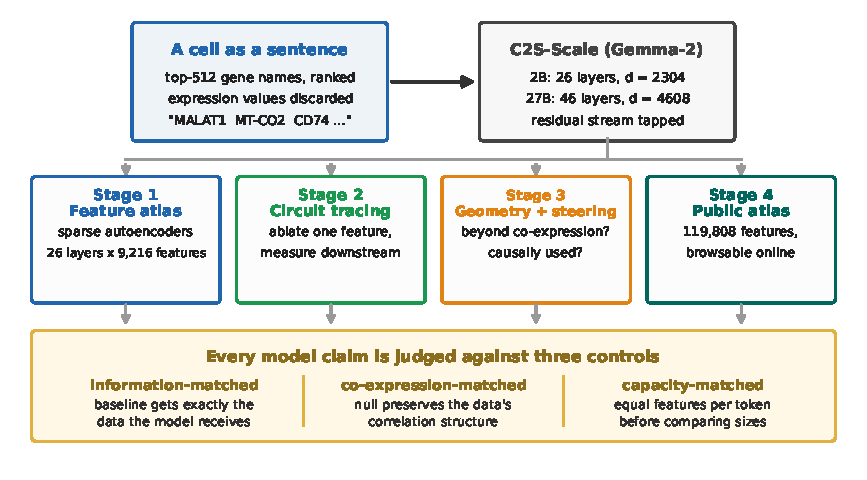
\includegraphics[width=\linewidth]{figures/fig1_design.pdf}
\caption{\textbf{The interpretability protocol and its application.} A cell is converted to a
sentence of the top-512 gene symbols in rank order, with expression magnitudes discarded, and passed
to C2S-Scale (Gemma-2, 2B and 27B). The residual stream is tapped and analysed in four stages: a
sparse-autoencoder feature atlas, causal circuit tracing, a regulatory-logic test, a
capacity-matched scaling control, geometry and steering tests, and public deployment. All model
claims are judged against expression baselines encoded with the same information the model
receives.}
\label{fig:design}
\end{figure}

\begin{figure}[htbp]\centering
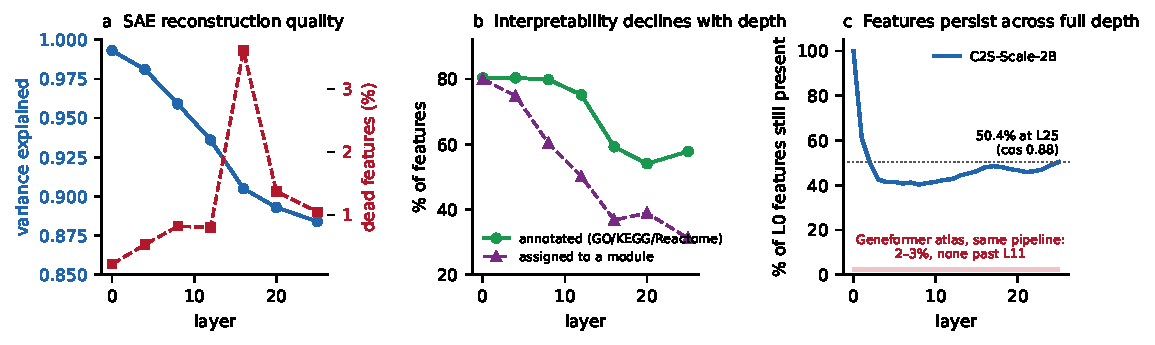
\includegraphics[width=\linewidth]{figures/fig2_sae_atlas.pdf}
\caption{\textbf{Sparse-autoencoder feature atlas of C2S-Scale-2B across all 26 layers.}
(a) Reconstruction quality: variance explained (left axis, blue) and dead features (right axis,
red). (b) Percentage of features receiving a significant ontology annotation (green) and assigned to
a co-activation module (purple). (c) Fraction of layer-0 features still recoverable at each later
layer by decoder cosine matching; the shaded band shows the 2--3\% retained by an encoder-style
single-cell model under the identical pipeline.}
\label{fig:atlas}
\end{figure}

\begin{figure}[htbp]\centering
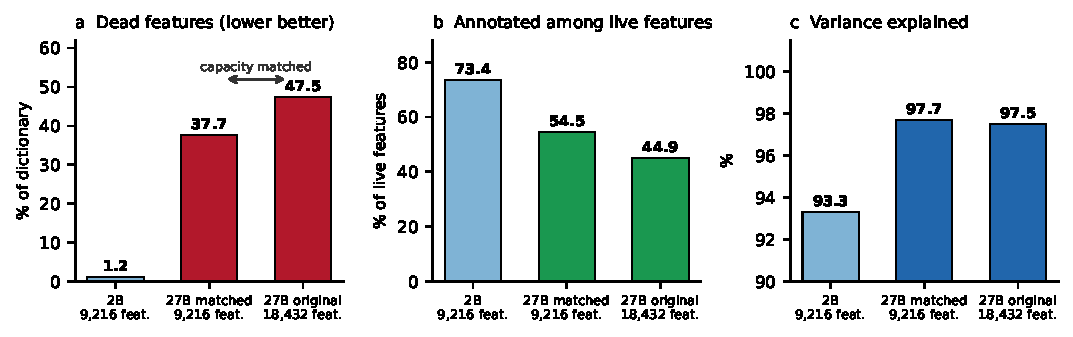
\includegraphics[width=\linewidth]{figures/fig3_scaling.pdf}
\caption{\textbf{Capacity-matched scaling control.} (a) Dead features, (b) percentage of live
features receiving an ontology annotation, and (c) variance explained, for the 2B model at
$4\times$ expansion, the 27B model retrained at $2\times$ expansion (matched to the same absolute
dictionary size and therefore the same positions per feature), and the 27B model at its native
$4\times$ expansion. Matching capacity recovers roughly ten points on each interpretability measure
but leaves a large gap.}
\label{fig:scaling}
\end{figure}

\begin{figure}[htbp]\centering
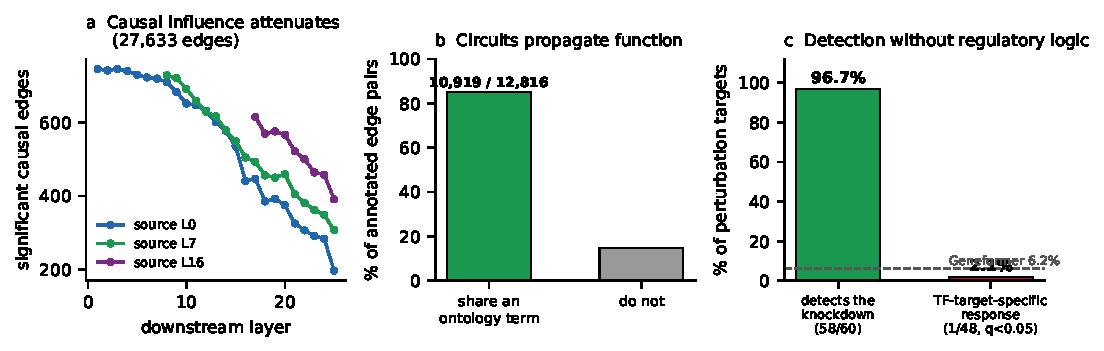
\includegraphics[width=\linewidth]{figures/fig4_circuits.pdf}
\caption{\textbf{Causal circuit tracing and the regulatory-logic test.} (a) Number of significant
causal edges from each source layer into each downstream layer; influence attenuates smoothly with
distance. (b) Of edges whose endpoints are both annotated, the proportion sharing at least one
ontology term. (c) Perturbation response: the model registers the knockdown for 96.7\% of targets
but only 2.1\% of transcription factors produce a target-specific response; the dashed line marks
the corresponding rate for an encoder-style reference model.}
\label{fig:circuits}
\end{figure}

\begin{figure}[htbp]\centering
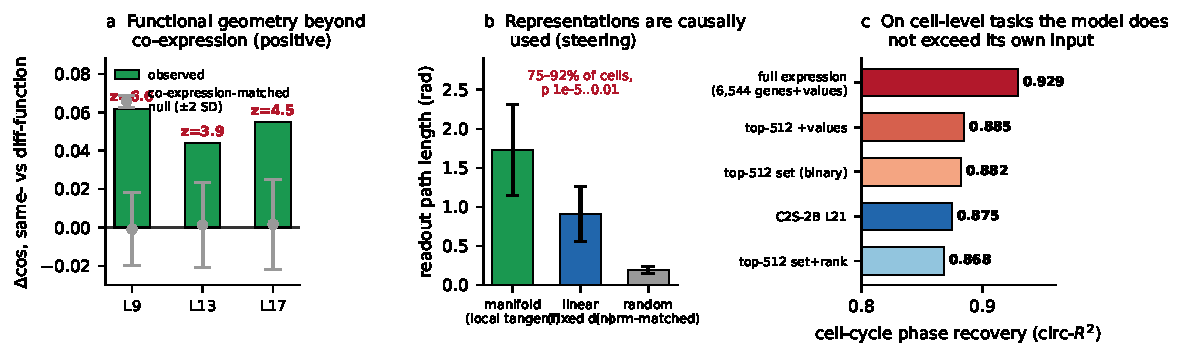
\includegraphics[width=\linewidth]{figures/fig5_beyond_input.pdf}
\caption{\textbf{What lies beyond the input.} (a) Within bins matched on co-expression and mean
expression, same-function gene pairs are more aligned than different-function pairs; grey points
show the co-expression-matched permutation null ($\pm 2$\,SD) and $z$-scores are given above each
bar. (b) Readout path length under three steering rules, in three independent runs; displacement
along the local geometry moves the model's own predictions further than a fixed linear direction,
while a norm-matched random direction does almost nothing. (c) Recovery of a cell-state variable
from full expression, from progressively more restricted encodings of the same data, and from the
model; the model sits within 0.007 of a linear readout of its own input encoding.}
\label{fig:beyond}
\end{figure}

\clearpage

\section*{References}
\begin{thebibliography}{99}
\bibitem{ref3} C.V. Theodoris, L. Xiao, A. Chopra, et al. (11 authors), Transfer learning enables predictions in network biology, Nature 618 (2023) 616--624. \url{https://doi.org/10.1038/s41586-023-06139-9}.
\bibitem{ref4} H. Cui, C. Wang, H. Maan, K. Pang, F. Luo, N. Duan, B. Wang, scGPT: toward building a foundation model for single-cell multi-omics using generative AI, Nat. Methods 21 (2024) 1470--1480. \url{https://doi.org/10.1038/s41592-024-02201-0}.
\bibitem{ref8} I. Kendiukhov, Systematic evaluation of single-cell foundation model interpretability reveals attention captures co-expression rather than unique regulatory signal, arXiv:2602.17532 (2026), preprint. \url{https://arxiv.org/abs/2602.17532}.
\bibitem{ref9} I. Kendiukhov, Systematic evaluation of single-cell foundation model interpretability: attention-derived edge scores add no incremental value over gene-level features for perturbation-target prediction, BMC Genomics 27 (2026). \url{https://doi.org/10.1186/s12864-026-12965-8}.
\bibitem{ref1} D. Levine, S.A. Rizvi, S. Lévy, et al. (19 authors), Cell2Sentence: teaching large language models the language of biology, in: Proc. 41st Int. Conf. Mach. Learn. (ICML), PMLR 235 (2024) 27299--27325. \url{https://proceedings.mlr.press/v235/levine24a.html}.
\bibitem{ref2} S.A. Rizvi, D. Levine, A. Patel, et al. (28 authors), Scaling large language models for next-generation single-cell analysis, bioRxiv preprint v4 (2026). \url{https://doi.org/10.1101/2025.04.14.648850}.
\bibitem{ref24} J.M. Replogle, R.A. Saunders, A.N. Pogson, et al. (17 authors), Mapping information-rich genotype-phenotype landscapes with genome-scale Perturb-seq, Cell 185 (2022) 2559--2575.e28. \url{https://doi.org/10.1016/j.cell.2022.05.013}.
\bibitem{ref25} M. Setty, V. Kiseliovas, J. Levine, A. Gayoso, L. Mazutis, D. Pe'er, Characterization of cell fate probabilities in single-cell data with Palantir, Nat. Biotechnol. 37 (2019) 451--460. \url{https://doi.org/10.1038/s41587-019-0068-4}.
\bibitem{ref21} N. Elhage, T. Hume, C. Olsson, et al. (16 authors), Toy models of superposition, Transformer Circuits Thread (2022). \url{https://transformer-circuits.pub/2022/toy_model/index.html} (accessed 18 August 2026).
\bibitem{ref17} T. Bricken, A. Templeton, J. Batson, et al. (24 authors), Towards monosemanticity: decomposing language models with dictionary learning, Transformer Circuits Thread (2023). \url{https://transformer-circuits.pub/2023/monosemantic-features/index.html} (accessed 18 August 2026).
\bibitem{ref18} A. Templeton, T. Conerly, J. Marcus, et al. (26 authors), Scaling monosemanticity: extracting interpretable features from Claude 3 Sonnet, Transformer Circuits Thread (2024). \url{https://transformer-circuits.pub/2024/scaling-monosemanticity/index.html} (accessed 18 August 2026).
\bibitem{ref19} H. Cunningham, A. Ewart, L. Riggs, R. Huben, L. Sharkey, Sparse autoencoders find highly interpretable features in language models, arXiv:2309.08600 (2023), preprint. \url{https://arxiv.org/abs/2309.08600}.
\bibitem{ref20} L. Gao, T. Dupré la Tour, H. Tillman, G. Goh, R. Troll, A. Radford, I. Sutskever, J. Leike, J. Wu, Scaling and evaluating sparse autoencoders, arXiv:2406.04093 (2024), preprint. \url{https://arxiv.org/abs/2406.04093}.
\bibitem{ref6} I. Kendiukhov, Sparse autoencoders reveal interpretable cell-type programs in single-cell foundation model representations, J. Biomed. Inform. 180 (2026) 105056. \url{https://doi.org/10.1016/j.jbi.2026.105056}.
\bibitem{ref7} I. Kendiukhov, Sparse autoencoders reveal organized biological knowledge but minimal regulatory logic in single-cell foundation models: a comparative atlas of Geneformer and scGPT, arXiv:2603.02952 (2026), preprint. \url{https://arxiv.org/abs/2603.02952}.
\bibitem{ref10} I. Kendiukhov, Causal circuit tracing reveals distinct computational architectures in single-cell foundation models: inhibitory dominance, biological coherence, and cross-model convergence, Bioinformatics 42 (2026) btag379. \url{https://doi.org/10.1093/bioinformatics/btag379}.
\bibitem{ref11} I. Kendiukhov, Exhaustive circuit mapping of a single-cell foundation model reveals massive redundancy, heavy-tailed hub architecture, and layer-dependent differentiation control, arXiv:2603.11940 (2026), preprint. \url{https://arxiv.org/abs/2603.11940}.
\bibitem{ref12} I. Kendiukhov, What topological and geometric structure do biological foundation models learn? Evidence from 141 hypotheses, PLOS ONE 21 (2026) e0344826. \url{https://doi.org/10.1371/journal.pone.0344826}.
\bibitem{ref13} I. Kendiukhov, Residual-stream geometry of single-cell foundation models carries incremental gene-regulatory signal across tissues, BMC Bioinformatics 27 (2026). \url{https://doi.org/10.1186/s12859-026-06538-5}.
\bibitem{ref37} I. Kendiukhov, Multi-dimensional spectral geometry of biological knowledge in single-cell transformer representations, arXiv:2602.22247 (2026), preprint. \url{https://arxiv.org/abs/2602.22247}.
\bibitem{ref14} I. Kendiukhov, Causal intervention validation of gene regulatory signals in scGPT, J. Biomed. Inform. 180 (2026) 105080. \url{https://doi.org/10.1016/j.jbi.2026.105080}.
\bibitem{ref5} K.Z. Kedzierska, L. Crawford, A.P. Amini, A.X. Lu, Zero-shot evaluation reveals limitations of single-cell foundation models, Genome Biol. 26 (2025) 101. \url{https://doi.org/10.1186/s13059-025-03574-x}.
\bibitem{ref39} I. Kendiukhov, Partial-label metric ceilings for evaluating gene regulatory networks inferred from single-cell foundation models, BioSystems 266 (2026) 105864. \url{https://doi.org/10.1016/j.biosystems.2026.105864}.
\bibitem{ref40} I. Kendiukhov, Quantifying ranking instability across evaluation protocol axes in gene regulatory network benchmarking, arXiv:2603.03493 (2026), preprint. \url{https://arxiv.org/abs/2603.03493}.
\bibitem{ref23} Gemma Team, M. Riviere, S. Pathak, et al., Gemma 2: improving open language models at a practical size, arXiv:2408.00118 (2024), preprint. \url{https://arxiv.org/abs/2408.00118}.
\bibitem{ref41} M. Ashburner, C.A. Ball, J.A. Blake, et al. (20 authors), Gene Ontology: tool for the unification of biology, Nat. Genet. 25 (2000) 25--29. \url{https://doi.org/10.1038/75556}.
\bibitem{ref42} The Gene Ontology Consortium, The Gene Ontology knowledgebase in 2026, Nucleic Acids Res. 54 (2026) D1779--D1792. \url{https://doi.org/10.1093/nar/gkaf1292}.
\bibitem{ref43} M. Kanehisa, S. Goto, KEGG: Kyoto Encyclopedia of Genes and Genomes, Nucleic Acids Res. 28 (2000) 27--30. \url{https://doi.org/10.1093/nar/28.1.27}.
\bibitem{ref44} M. Kanehisa, M. Furumichi, Y. Sato, Y. Matsuura, M. Ishiguro-Watanabe, KEGG: biological systems database as a model of the real world, Nucleic Acids Res. 53 (2025) D672--D677. \url{https://doi.org/10.1093/nar/gkae909}.
\bibitem{ref45} E. Ragueneau, C. Gong, P. Sinquin, et al. (25 authors), The Reactome Knowledgebase 2026, Nucleic Acids Res. 54 (2026) D673--D681. \url{https://doi.org/10.1093/nar/gkaf1223}.
\bibitem{ref46} D. Szklarczyk, K. Nastou, M. Koutrouli, et al. (15 authors), The STRING database in 2025: protein networks with directionality of regulation, Nucleic Acids Res. 53 (2025) D730--D737. \url{https://doi.org/10.1093/nar/gkae1113}.
\bibitem{ref47} H. Han, J.-W. Cho, S. Lee, et al. (20 authors), TRRUST v2: an expanded reference database of human and mouse transcriptional regulatory interactions, Nucleic Acids Res. 46 (2018) D380--D386. \url{https://doi.org/10.1093/nar/gkx1013}.
\bibitem{ref34} Y. Benjamini, Y. Hochberg, Controlling the false discovery rate: a practical and powerful approach to multiple testing, J. R. Stat. Soc. Ser. B Methodol. 57 (1995) 289--300. \url{https://doi.org/10.1111/j.2517-6161.1995.tb02031.x}.
\bibitem{ref32} V.A. Traag, L. Waltman, N.J. van Eck, From Louvain to Leiden: guaranteeing well-connected communities, Sci. Rep. 9 (2019) 5233. \url{https://doi.org/10.1038/s41598-019-41695-z}.
\bibitem{ref22} K. Meng, D. Bau, A. Andonian, Y. Belinkov, Locating and editing factual associations in GPT, in: Adv. Neural Inf. Process. Syst. 35 (NeurIPS 2022), 2022. \url{https://arxiv.org/abs/2202.05262}.
\bibitem{ref48} A.M. Turner, L. Thiergart, G. Leech, D. Udell, J.J. Vazquez, U. Mini, M. MacDiarmid, Steering language models with activation engineering, arXiv:2308.10248 (2023), preprint. \url{https://arxiv.org/abs/2308.10248}.
\bibitem{ref49} A. Zou, L. Phan, S. Chen, et al. (21 authors), Representation engineering: a top-down approach to AI transparency, arXiv:2310.01405 (2023), preprint. \url{https://arxiv.org/abs/2310.01405}.
\bibitem{ref50} L. McInnes, J. Healy, J. Melville, UMAP: uniform manifold approximation and projection for dimension reduction, arXiv:1802.03426 (2018), preprint. \url{https://arxiv.org/abs/1802.03426}.
\end{thebibliography}

\end{document}
